\begin{frame}{Algorithmus von Feldmann und Foschini}
    Fast ausgewogene Partitionierung auf Bäumen mit $\alpha=1$\\
    \pause
    Zweiphasig:
    \begin{itemize}[<+(1)->]
        \item Schnittphase
        \item Packphase
    \end{itemize}
\end{frame}

\begin{frame}[fragile]{Zerlegung in Zusammenhangskomponenten}
    \begin{center}
        \begin{tikzpicture}[
            randomdraw/.style={decoration={random steps, segment length=8pt, amplitude=3pt}},
            every node/.style={scale=0.7},
            ampersand replacement=\&
        ]

            \pgfmathsetseed{23654}
            \coordinate (A) at (0.0,0.0);
            \coordinate (B) at (2.0,0.0);
            \coordinate (C) at (1.0,1.5);
            \coordinate (D) at (0.0,3.0);
            \coordinate (E) at (-1.0,1.5);
            \coordinate (F) at (-2.0,0.0);

            \node[align=left] at (1.75, 2.5) {$n=50$\\$k=4$\\$\ceil{n/k}=13$};
                
            \draw (A) -- coordinate[midway](AB) (B) -- coordinate[midway](BC) (C)
                -- coordinate[midway](CD) (D) -- coordinate[near end](DE) (E)
                -- coordinate[near start](EF) (F) -- coordinate[midway](FA) (A);
            \draw (B) -- coordinate[near end](BCM) (C);

            \visible<2->{
                \draw decorate[randomdraw]{(AB) -- (DE)};
                \draw decorate[randomdraw]{(FA) -- (C)};
            }
            \visible<3->{
                \draw decorate[randomdraw]{(EF) -- (A)};
                \draw decorate[randomdraw]{(DE) -- (CD)};
            }
            \visible<4->{
                \draw decorate[randomdraw]{(E) -- (C)};
                \draw decorate[randomdraw]{(AB) -- (BC)};
                \draw decorate[randomdraw]{(A) -- (BCM)};
            }

            \visible<5->{
                \node at (0.0,2.5) {$6$};
                \node at (0.25,1.75) {$7$};
                \node at (0.25,1.25) {$4$};
                \node at (0.75,1.0) {$3$};
                \node at (1.0,0.6125) {$3$};
                \node at (1.5,0.25) {$4$};
                \node at (0.0,0.5) {$4$};
                \node at (0.5,0.125) {$2$};
                \node at (-0.5,0.125) {$2$};
                \node at (-0.5,1.0) {$6$};
                \node at (-1.25,0.5) {$7$};
                \node at (-0.68,1.6125) {$2$};
            }
            
            %\draw[help lines] (F) grid[step=0.25] (2.0,3.0);

            \visible<6->{
		        \matrix[
                    matrix of nodes,
                    nodes={align=center,text width=0.4cm},
                ] at (0.0, -1.0) (dict) {
                    $1$ \& $2$ \& $3$ \& $4$ \& $5$ \& $6$ \& $7$ \& $8$ \& $9$ \& $10$ \& $11$ \& $12$ \& $13$ \\
                    $0$ \& $3$ \& $2$ \& $3$ \& $0$ \& $2$ \& $2$ \& $0$ \& $0$ \& $0$ \& $0$ \& $0$ \& $0$ \\
                };
                \draw (dict-1-1.south west) -- (dict-1-13.south east);
            }
        

        \end{tikzpicture}
    \end{center}
\end{frame}

\begin{frame}[fragile]{Berechnung der Repräsentanten}
    \begin{center}
        \begin{tikzpicture}[
            randomdraw/.style={decoration={random steps, segment length=8pt, amplitude=3pt}},
            every node/.style={scale=0.7}
        ]

            \pgfmathsetseed{23654}
            \begin{scope}[shift={(0.0,2.5)}, xscale=0.7, yscale=0.7, every node/.style={scale=0.55}]
                \coordinate (A) at (0.0,0.0);
                \coordinate (B) at (2.0,0.0);
                \coordinate (C) at (1.0,1.5);
                \coordinate (D) at (0.0,3.0);
                \coordinate (E) at (-1.0,1.5);
                \coordinate (F) at (-2.0,0.0);

                \node[align=left] at (1.75, 2.4) {$n=50$\\$k=4$\\$\ceil{n/k}=13$};

                \draw (A) -- coordinate[midway](AB) (B) -- coordinate[midway](BC) (C)
                    -- coordinate[midway](CD) (D) -- coordinate[near end](DE) (E)
                    -- coordinate[near start](EF) (F) -- coordinate[midway](FA) (A);
                \draw (B) -- coordinate[near end](BCM) (C);

                \visible<2->{
                    \draw[line width=1pt, TUMAccentOrange] (F) -- (B) -- (D) -- cycle;
                    \path (F) -- node[sloped, yshift=12pt, midway]{Minimale Schnittkosten} (D);
                }


                \draw decorate[randomdraw]{(AB) -- (DE)};
                \draw decorate[randomdraw]{(FA) -- (C)};
                \draw decorate[randomdraw]{(EF) -- (A)};
                \draw decorate[randomdraw]{(DE) -- (CD)};
                \draw decorate[randomdraw]{(E) -- (C)};
                \draw decorate[randomdraw]{(AB) -- (BC)};
                \draw decorate[randomdraw]{(A) -- (BCM)};

                \node at (0.0,2.5) {$6$};
                \node at (0.25,1.75) {$7$};
                \node at (0.25,1.25) {$4$};
                \node at (0.75,1.0) {$3$};
                \node at (1.0,0.57) {$3$};
                \node at (1.5,0.25) {$4$};
                \node at (0.0,0.42) {$4$};
                \node at (0.6,0.17) {$2$};
                \node at (-0.5,0.17) {$2$};
                \node at (-0.5,1.0) {$6$};
                \node at (-1.25,0.5) {$7$};
                \node at (-0.73,1.6125) {$2$};

                %\draw[help lines] (F) grid[step=0.25] (2.0,3.0);

                \matrix(dict)[
                    matrix of nodes,
                    nodes={align=center,text width=0.4cm},
                ] at (0.0, -1.0) {
                    $1$ & $2$ & $3$ & $4$ & $5$ & $6$ & $7$ & $8$ & $9$ & $10$ & $11$ & $12$ & $13$ \\
                    $0$ & $3$ & $2$ & $3$ & $0$ & $2$ & $2$ & $0$ & $0$ & $0$ & $0$ & $0$ & $0$ \\
                };
                \draw(dict-1-1.south west)--(dict-1-13.south east);
            \end{scope}

            \begin{scope}[shift={(-2.75,-0.75)}, xscale=-0.7, yscale=0.7, every node/.style={scale=0.4}]
                \coordinate (A) at (0.0,0.0);
                \coordinate (B) at (2.0,0.0);
                \coordinate (C) at (1.0,1.5);
                \coordinate (D) at (0.0,3.0);
                \coordinate (E) at (-1.0,1.5);
                \coordinate (F) at (-2.0,0.0);

                \draw (A) -- coordinate[midway](AB) (B) -- coordinate[midway](BC) (C)
                    -- coordinate[midway](CD) (D) -- coordinate[near end](DE) (E)
                    -- coordinate[near start](EF) (F) -- coordinate[midway](FA) (A);
                \draw (B) -- coordinate[near end](BCM) (C);

                \draw decorate[randomdraw]{(AB) -- (DE)};
                \draw decorate[randomdraw]{(FA) -- (C)};
                \draw decorate[randomdraw]{(EF) -- (A)};
                \draw decorate[randomdraw]{(DE) -- (CD)};
                \draw decorate[randomdraw]{(E) -- (C)};
                \draw decorate[randomdraw]{(AB) -- (BC)};
                \draw decorate[randomdraw]{(A) -- (BCM)};

                %\draw[help lines] (F) grid[step=0.25] (2.0,3.0);

            \end{scope}

            \begin{scope}[shift={(2.75,-0.75)}, xscale=0.7, yscale=0.7, every node/.style={scale=0.4}]
                \coordinate (A) at (0.0,0.0);
                \coordinate (B) at (2.0,0.0);
                \coordinate (C) at (1.0,1.5);
                \coordinate (D) at (0.0,3.0);
                \coordinate (E) at (-1.0,1.5);
                \coordinate (F) at (-2.0,0.0);

                \draw (A) -- coordinate[midway](AB) (B) -- coordinate[midway](BC) (C)
                    -- coordinate[midway](CD) (D) -- coordinate[near end](DE) (E)
                    -- coordinate[near start](EF) (F) -- coordinate[midway](FA) (A);
                \draw (B) -- coordinate[near end](BCM) (C);

                \draw decorate[randomdraw]{(AB) -- (DE)};
                \draw decorate[randomdraw]{(FA) -- (C)};
                \draw decorate[randomdraw]{(EF) -- (A)};
                \draw decorate[randomdraw]{(DE) -- (CD)};
                \draw decorate[randomdraw]{(E) -- (C)};
                \draw decorate[randomdraw]{(AB) -- (BC)};
                \draw decorate[randomdraw]{(A) -- (BCM)};

                %\draw[help lines] (F) grid[step=0.25] (2.0,3.0);

            \end{scope}

            \draw [line width=1.0pt, black] (0.0,1.0) ellipse (5.2cm and 3.8cm);

        \end{tikzpicture}
    \end{center}
\end{frame}

\begin{frame}[fragile]{Unterteilung in Äquivalenzklassen}
    \vspace{-0.5cm}
    \begin{center}
        \begin{tikzpicture}[
            randomdraw/.style={decoration={random steps, segment length=8pt, amplitude=3pt}},
            every node/.style={scale=0.7}
        ]
            \pgfmathsetseed{23654}

            \begin{scope}[shift={(0.0,3.5)}, xscale=0.5, yscale=0.5]
                \begin{scope}[shift={(0.0,2.5)}, xscale=0.7, yscale=0.7, every node/.style={scale=0.42}]
                    \coordinate (A) at (0.0,0.0);
                    \coordinate (B) at (2.0,0.0);
                    \coordinate (C) at (1.0,1.5);
                    \coordinate (D) at (0.0,3.0);
                    \coordinate (E) at (-1.0,1.5);
                    \coordinate (F) at (-2.0,0.0);

                    \draw (A) -- coordinate[midway](AB) (B) -- coordinate[midway](BC) (C)
                        -- coordinate[midway](CD) (D) -- coordinate[near end](DE) (E)
                        -- coordinate[near start](EF) (F) -- coordinate[midway](FA) (A);
                    \draw (B) -- coordinate[near end](BCM) (C);

                    \draw[line width=1pt, TUMAccentOrange] (F) -- (B) -- (D) -- cycle;
                    \path (F) -- node[sloped, yshift=9pt, xshift=-2pt, midway]{\scriptsize Minimale Schnittkosten} (D);


                    \draw decorate[randomdraw]{(AB) -- (DE)};
                    \draw decorate[randomdraw]{(FA) -- (C)};
                    \draw decorate[randomdraw]{(EF) -- (A)};
                    \draw decorate[randomdraw]{(DE) -- (CD)};
                    \draw decorate[randomdraw]{(E) -- (C)};
                    \draw decorate[randomdraw]{(AB) -- (BC)};
                    \draw decorate[randomdraw]{(A) -- (BCM)};

                    %\draw[help lines] (F) grid[step=0.25] (2.0,3.0);

                    \matrix(dict)[
                        matrix of nodes,
                        nodes={align=center,text width=0.4cm},
                    ] at (0.0, -1.0) {
                        $1$ & $2$ & $3$ & $4$ & $5$ & $6$ & $7$ & $8$ & $9$ & $10$ & $11$ & $12$ & $13$ \\
                        $0$ & $3$ & $2$ & $3$ & $0$ & $2$ & $2$ & $0$ & $0$ & $0$ & $0$ & $0$ & $0$ \\
                    };
                    \draw(dict-1-1.south west)--(dict-1-13.south east);
                \end{scope}

                \begin{scope}[shift={(-2.75,-0.75)}, xscale=-0.7, yscale=0.7, every node/.style={scale=0.4}]
                    \coordinate (A) at (0.0,0.0);
                    \coordinate (B) at (2.0,0.0);
                    \coordinate (C) at (1.0,1.5);
                    \coordinate (D) at (0.0,3.0);
                    \coordinate (E) at (-1.0,1.5);
                    \coordinate (F) at (-2.0,0.0);

                    \draw (A) -- coordinate[midway](AB) (B) -- coordinate[midway](BC) (C)
                        -- coordinate[midway](CD) (D) -- coordinate[near end](DE) (E)
                        -- coordinate[near start](EF) (F) -- coordinate[midway](FA) (A);
                    \draw (B) -- coordinate[near end](BCM) (C);

                    \draw decorate[randomdraw]{(AB) -- (DE)};
                    \draw decorate[randomdraw]{(FA) -- (C)};
                    \draw decorate[randomdraw]{(EF) -- (A)};
                    \draw decorate[randomdraw]{(DE) -- (CD)};
                    \draw decorate[randomdraw]{(E) -- (C)};
                    \draw decorate[randomdraw]{(AB) -- (BC)};
                    \draw decorate[randomdraw]{(A) -- (BCM)};

                    %\draw[help lines] (F) grid[step=0.25] (2.0,3.0);

                \end{scope}

                \begin{scope}[shift={(2.75,-0.75)}, xscale=0.7, yscale=0.7, every node/.style={scale=0.4}]
                    \coordinate (A) at (0.0,0.0);
                    \coordinate (B) at (2.0,0.0);
                    \coordinate (C) at (1.0,1.5);
                    \coordinate (D) at (0.0,3.0);
                    \coordinate (E) at (-1.0,1.5);
                    \coordinate (F) at (-2.0,0.0);

                    \draw (A) -- coordinate[midway](AB) (B) -- coordinate[midway](BC) (C)
                        -- coordinate[midway](CD) (D) -- coordinate[near end](DE) (E)
                        -- coordinate[near start](EF) (F) -- coordinate[midway](FA) (A);
                    \draw (B) -- coordinate[near end](BCM) (C);

                    \draw decorate[randomdraw]{(AB) -- (DE)};
                    \draw decorate[randomdraw]{(FA) -- (C)};
                    \draw decorate[randomdraw]{(EF) -- (A)};
                    \draw decorate[randomdraw]{(DE) -- (CD)};
                    \draw decorate[randomdraw]{(E) -- (C)};
                    \draw decorate[randomdraw]{(AB) -- (BC)};
                    \draw decorate[randomdraw]{(A) -- (BCM)};

                    %\draw[help lines] (F) grid[step=0.25] (2.0,3.0);

                \end{scope}

                \draw [line width=1.0pt, black] (0.0,1.0) ellipse (5.2cm and 3.8cm);
            \end{scope}

            % SECOND
            \begin{scope}[shift={(-3.0,0.0)}, xscale=0.5, yscale=0.5]
                \begin{scope}[shift={(0.0,2.5)}, xscale=0.7, yscale=0.7, every node/.style={scale=0.42}]
                    \coordinate (A) at (0.0,0.0);
                    \coordinate (B) at (2.0,0.0);
                    \coordinate (C) at (1.0,1.5);
                    \coordinate (D) at (0.0,3.0);
                    \coordinate (E) at (-1.0,1.5);
                    \coordinate (F) at (-2.0,0.0);

                    \draw (A) -- coordinate[midway](AB) (B) -- coordinate[midway](BC) (C)
                        -- coordinate[midway](CD) (D) -- coordinate[near end](DE) (E)
                        -- coordinate[near start](EF) (F) -- coordinate[midway](FA) (A);
                    \draw (B) -- coordinate[near end](BCM) (C);

                    \draw[line width=1pt, TUMAccentOrange] (F) -- (B) -- (D) -- cycle;
                    \path (F) -- node[sloped, yshift=9pt, xshift=-2pt, midway]{\scriptsize Minimale Schnittkosten} (D);


                    \draw decorate[randomdraw]{(AB) -- (DE)};
                    \draw decorate[randomdraw]{(FA) -- (C)};
                    \draw decorate[randomdraw]{(D) -- (A)};
                    \draw decorate[randomdraw]{(A) -- (EF)};
                    \draw decorate[randomdraw]{(EF) -- (FA)};
                    \draw decorate[randomdraw]{(DE) -- (CD)};
                    \draw decorate[randomdraw]{(CD) -- (EF)};
                    \draw decorate[randomdraw]{(AB) -- (BC)};
                    \draw decorate[randomdraw]{(A) -- (BCM)};

                    %\draw[help lines] (F) grid[step=0.25] (2.0,3.0);

                    \matrix(dict)[
                        matrix of nodes,
                        nodes={align=center,text width=0.4cm},
                    ] at (0.0, -1.0) {
                        $1$ & $2$ & $3$ & $4$ & $5$ & $6$ & $7$ & $8$ & $9$ & $10$ & $11$ & $12$ & $13$ \\
                        $2$ & $5$ & $4$ & $2$ & $2$ & $0$ & $1$ & $0$ & $1$ & $0$ & $0$ & $0$ & $0$ \\
                    };
                    \draw(dict-1-1.south west)--(dict-1-13.south east);
                \end{scope}

                \begin{scope}[shift={(-2.75,-0.75)}, xscale=-0.7, yscale=0.7, every node/.style={scale=0.4}]
                    \coordinate (A) at (0.0,0.0);
                    \coordinate (B) at (2.0,0.0);
                    \coordinate (C) at (1.0,1.5);
                    \coordinate (D) at (0.0,3.0);
                    \coordinate (E) at (-1.0,1.5);
                    \coordinate (F) at (-2.0,0.0);

                    \draw (A) -- coordinate[midway](AB) (B) -- coordinate[midway](BC) (C)
                        -- coordinate[midway](CD) (D) -- coordinate[near end](DE) (E)
                        -- coordinate[near start](EF) (F) -- coordinate[midway](FA) (A);
                    \draw (B) -- coordinate[near end](BCM) (C);

                    %\draw[help lines] (F) grid[step=0.25] (2.0,3.0);
                    \draw decorate[randomdraw]{(AB) -- (DE)};
                    \draw decorate[randomdraw]{(FA) -- (C)};
                    \draw decorate[randomdraw]{(EF) -- (A)};
                    \draw decorate[randomdraw]{(EF) -- (FA)};
                    \draw decorate[randomdraw]{(DE) -- (CD)};
                    \draw decorate[randomdraw]{(E) -- (C)};
                    \draw decorate[randomdraw]{(AB) -- (BC)};
                    \draw decorate[randomdraw]{(A) -- (BCM)};
                    \draw decorate[randomdraw]{(D) -- (A)};

                \end{scope}

                \begin{scope}[shift={(2.75,-0.75)}, xscale=0.7, yscale=0.7, every node/.style={scale=0.4}]
                    \coordinate (A) at (0.0,0.0);
                    \coordinate (B) at (2.0,0.0);
                    \coordinate (C) at (1.0,1.5);
                    \coordinate (D) at (0.0,3.0);
                    \coordinate (E) at (-1.0,1.5);
                    \coordinate (F) at (-2.0,0.0);

                    \draw (A) -- coordinate[midway](AB) (B) -- coordinate[midway](BC) (C)
                        -- coordinate[midway](CD) (D) -- coordinate[near end](DE) (E)
                        -- coordinate[near start](EF) (F) -- coordinate[midway](FA) (A);
                    \draw (B) -- coordinate[near end](BCM) (C);

                    %\draw[help lines] (F) grid[step=0.25] (2.0,3.0);
                    \draw decorate[randomdraw]{(AB) -- (DE)};
                    \draw decorate[randomdraw]{(FA) -- (C)};
                    \draw decorate[randomdraw]{(EF) -- (A)};
                    \draw decorate[randomdraw]{(EF) -- (FA)};
                    \draw decorate[randomdraw]{(DE) -- (CD)};
                    \draw decorate[randomdraw]{(D) -- (A)};
                    \draw decorate[randomdraw]{(E) -- (C)};
                    \draw decorate[randomdraw]{(AB) -- (BC)};
                    \draw decorate[randomdraw]{(BCM) -- (A)};

                \end{scope}

                \draw [line width=1.0pt, black] (0.0,1.0) ellipse (5.2cm and 3.8cm);
            \end{scope}

            % THIRD
            \begin{scope}[shift={(3.0,0.0)}, xscale=0.5, yscale=0.5]
                \begin{scope}[shift={(0.0,2.5)}, xscale=0.7, yscale=0.7, every node/.style={scale=0.42}]
                    \coordinate (A) at (0.0,0.0);
                    \coordinate (B) at (2.0,0.0);
                    \coordinate (C) at (1.0,1.5);
                    \coordinate (D) at (0.0,3.0);
                    \coordinate (E) at (-1.0,1.5);
                    \coordinate (F) at (-2.0,0.0);

                    \draw (A) -- coordinate[midway](AB) (B) -- coordinate[midway](BC) (C)
                        -- coordinate[midway](CD) (D) -- coordinate[near end](DE) (E)
                        -- coordinate[near start](EF) (F) -- coordinate[midway](FA) (A);
                    \draw (B) -- coordinate[near end](BCM) (C);

                    \draw[line width=1pt, TUMAccentOrange] (F) -- (B) -- (D) -- cycle;
                    \path (F) -- node[sloped, yshift=9pt, xshift=-2pt, midway]{\scriptsize Minimale Schnittkosten} (D);


                    \draw decorate[randomdraw]{(F) -- (C)};
                    \draw decorate[randomdraw]{(DE) -- (A)};
                    \draw decorate[randomdraw]{(C) -- (A)};

                    %\draw[help lines] (F) grid[step=0.25] (2.0,3.0);

                    \matrix(dict)[
                        matrix of nodes,
                        nodes={align=center,text width=0.4cm},
                    ] at (0.0, -1.0) {
                        $1$ & $2$ & $3$ & $4$ & $5$ & $6$ & $7$ & $8$ & $9$ & $10$ & $11$ & $12$ & $13$ \\
                        $0$ & $0$ & $0$ & $0$ & $0$ & $0$ & $0$ & $1$ & $0$ & $2$ & $2$ & $0$ & $0$ \\
                    };
                    \draw(dict-1-1.south west)--(dict-1-13.south east);
                \end{scope}

                \begin{scope}[shift={(-2.75,-0.75)}, xscale=-0.7, yscale=0.7, every node/.style={scale=0.4}]
                    \coordinate (A) at (0.0,0.0);
                    \coordinate (B) at (2.0,0.0);
                    \coordinate (C) at (1.0,1.5);
                    \coordinate (D) at (0.0,3.0);
                    \coordinate (E) at (-1.0,1.5);
                    \coordinate (F) at (-2.0,0.0);

                    \draw (A) -- coordinate[midway](AB) (B) -- coordinate[midway](BC) (C)
                        -- coordinate[midway](CD) (D) -- coordinate[near end](DE) (E)
                        -- coordinate[near start](EF) (F) -- coordinate[midway](FA) (A);
                    \draw (B) -- coordinate[near end](BCM) (C);

                    \draw decorate[randomdraw]{(F) -- (C)};
                    \draw decorate[randomdraw]{(DE) -- (A)};
                    \draw decorate[randomdraw]{(C) -- (A)};

                    %\draw[help lines] (F) grid[step=0.25] (2.0,3.0);

                \end{scope}

                \begin{scope}[shift={(2.75,-0.75)}, xscale=0.7, yscale=0.7, every node/.style={scale=0.4}]
                    \coordinate (A) at (0.0,0.0);
                    \coordinate (B) at (2.0,0.0);
                    \coordinate (C) at (1.0,1.5);
                    \coordinate (D) at (0.0,3.0);
                    \coordinate (E) at (-1.0,1.5);
                    \coordinate (F) at (-2.0,0.0);

                    \draw (A) -- coordinate[midway](AB) (B) -- coordinate[midway](BC) (C)
                        -- coordinate[midway](CD) (D) -- coordinate[near end](DE) (E)
                        -- coordinate[near start](EF) (F) -- coordinate[midway](FA) (A);
                    \draw (B) -- coordinate[near end](BCM) (C);

                    \draw decorate[randomdraw]{(C) -- (A)};
                    \draw decorate[randomdraw]{(F) -- (C)};
                    \draw decorate[randomdraw]{(A) -- (DE)};

                    %\draw[help lines] (F) grid[step=0.25] (2.0,3.0);

                \end{scope}

                \draw [line width=1.0pt, black] (0.0,1.0) ellipse (5.2cm and 3.8cm);
            \end{scope}
        \end{tikzpicture}
    \end{center}
\end{frame}

\begin{frame}[fragile]{Packen der Zusammenhangskomponenten}
    \begin{center}
        \begin{tikzpicture}[
            randomdraw/.style={decoration={random steps, segment length=8pt, amplitude=3pt}},
            every node/.style={scale=0.8},
            ampersand replacement=\&
        ]

            \pgfmathsetseed{23654}
            \coordinate (A) at (0.0,0.0);
            \coordinate (B) at (2.0,0.0);
            \coordinate (C) at (1.0,1.5);
            \coordinate (D) at (0.0,3.0);
            \coordinate (E) at (-1.0,1.5);
            \coordinate (F) at (-2.0,0.0);

            \node[align=left] at (1.75, 2.5) {$n=50$};
                
            \draw (A) -- coordinate[midway](AB) (B) -- coordinate[midway](BC) (C)
                -- coordinate[midway](CD) (D) -- coordinate[near end](DE) (E)
                -- coordinate[near start](EF) (F) -- coordinate[midway](FA) (A);
            \draw (B) -- coordinate[near end](BCM) (C);

            \draw[name path=ABDE, save path=\pathABDE] decorate[randomdraw]{(AB) -- (DE)};
            \draw[name path=FAC, save path=\pathFAC] decorate[randomdraw]{(FA) -- (C)};
            \draw[name path=EFA, save path=\pathEFA] decorate[randomdraw]{(EF) -- (A)};
            \draw[name path=DECD, save path=\pathDECD] decorate[randomdraw]{(DE) -- (CD)};
            \draw[name path=EC, save path=\pathEC] decorate[randomdraw]{(E) -- (C)};
            \draw[name path=ABBC, save path=\pathABBC] decorate[randomdraw]{(AB) -- (BC)};
            \draw[name path=ABCM, save path=\pathABCM] decorate[randomdraw]{(A) -- (BCM)};

            \path[name path=ECABDERTWO]
                [intersection segments={of=EC and ABDE, sequence={R1}}];
            \path[name path=EFAFACRTWO]
                [intersection segments={of=EFA and FAC, sequence={R2}}];
            \path[name path=PREVLONE]
                [intersection segments={of=ECABDERTWO and EFAFACRTWO, sequence={L1}}];

            \begin{scope}[on background layer]
                \visible<2->{
                    \fill[fill=TUMAccentBlue, intersection segments={
                        of=ABCM and ABDE, sequence={R1--L1[reverse]}}] -- cycle;
                    
                    \fill[fill=TUMAccentBlue]
                        [intersection segments={of=ECABDERTWO and EFAFACRTWO, sequence={L2[reverse]--R2}}]
                        [intersection segments={of=ABDE and EC, sequence={R2[reverse]}}]
                        ;

                    \fill[fill=TUMAccentBlue]
                        [intersection segments={of=PREVLONE and ABCM, sequence={R2[reverse]--L2}}]
                        [intersection segments={of=ECABDERTWO and EFAFACRTWO, sequence={R2}}] -- (BCM)
                        ;

                    \fill[fill=TUMAccentBlue]
                        [intersection segments={of=ABBC and ABBC, sequence={L*[reverse]}}]
                        [intersection segments={of=ECABDERTWO and ABCM, sequence={L1--R2}}] -- (BC);
                }

                \visible<3->{
                    \fill[fill=TUMAccentOrange, intersection segments={
                        of=ABDE and EC, sequence=L2--R1}];

                    \fill[fill=TUMAccentOrange, intersection segments={
                        of=FAC and EFA, sequence={L1--R2}}] -- cycle;

                    \fill[fill=TUMAccentOrange]
                        [intersection segments={of=ECABDERTWO and EFAFACRTWO, sequence={R1}}] -- (A)
                        [intersection segments={of=PREVLONE and ABCM, sequence={L2[reverse]--R1[reverse]}}]
                        [intersection segments={of=FAC and EFA, sequence={R2[reverse]}}]
                        ;

                }
                \makeatletter
                \pgfsyssoftpath@setcurrentpath{\pathABBC} \visible<3->{\filldraw[draw, fill=TUMAccentOrange] -- (B) -- cycle;}
                \makeatother


                \visible<4->{
                    \fill[fill=TUMAccentGreen, intersection segments={
                        of=EFA and FAC, sequence={L1--R1[reverse]}}] -- (F) -- cycle;

                    \fill[fill=TUMAccentGreen]
                        [intersection segments={of=EC and ABDE, sequence={L1}}]
                        [intersection segments={of=ECABDERTWO and EFAFACRTWO, sequence={L2[reverse] -- R1[reverse]}}] -- (E)
                        [intersection segments={of=EFA and FAC, sequence={L1[reverse]}}] -- (E)
                        ;
                }

                \visible<5->{
                    \fill[fill=TUMGray]
                        [intersection segments={of=EC and ABDE, sequence={L2[reverse] -- R2}}]
                        [intersection segments={of=DECD and DECD, sequence={L*}}] -- (C);

                }
                \makeatletter
                \pgfsyssoftpath@setcurrentpath{\pathDECD} \visible<5->{\filldraw[draw, fill=TUMGray] -- (D) -- cycle;}
                \makeatother

            \end{scope}

            \node at (0.0,2.5) {$6$};
            \node at (0.25,1.75) {$7$};
            \node at (0.25,1.25) {$4$};
            \node at (0.75,1.0) {$3$};
            \node at (1.0,0.6125) {$3$};
            \node at (1.5,0.25) {$4$};
            \node at (0.0,0.5) {$4$};
            \node at (0.5,0.125) {$2$};
            \node at (-0.5,0.125) {$2$};
            \node at (-0.5,1.0) {$6$};
            \node at (-1.25,0.5) {$7$};
            \node at (-0.68,1.6125) {$2$};
            
            %\draw[help lines] (F) grid[step=0.25] (2.0,3.0);

		    \matrix[
                matrix of nodes,
                nodes={align=center,text width=0.4cm},
            ] at (-5.5, 4.0) (dict) {
                $1$ \& $2$ \& $3$ \& $4$ \& $5$ \& $6$ \& $7$ \& $8$ \& $9$ \& $10$ \& $11$ \& $12$ \& $13$ \\
                $0$ \& $3$ \& $2$ \& $3$ \& $0$ \& $2$ \& $2$ \& $0$ \& $0$ \& $0$ \& $0$ \& $0$ \& $0$ \\
            };
            \draw (dict-1-1.south west) -- (dict-1-13.south east);
			
			\foreach \bin/\x in {ONE/-8.5,TWO/-7,THREE/-5.5,FOUR/-4}{
				\coordinate (\bin{}BL) at (\x,0);
				\coordinate (\bin{}BR) at ($ (\x,0) + (0.9,0.0) $);
				\coordinate (\bin{}TL) at ($ (\x,0) + (0.0,2.6) $);
				\coordinate (\bin{}TR) at ($ (\x,0) + (0.9,2.6) $);

                \draw[line width=1pt] (\bin{}TL) -- (\bin{}BL) -- (\bin{}BR) -- (\bin{}TR);
			}

            \begin{scope}[on background layer]
                \foreach \bin/\y/\s in {ONE/0/0.4,ONE/0.4/0.6,ONE/1.0/0.6,ONE/1.6/0.8}{
                    \visible<2->{\filldraw[draw=white, fill=TUMAccentBlue] ($ (\bin{}BL) + (0.0,\y) $) rectangle ($ (\bin{}BL) + (0.9,\y+\s) $);}
			    }

                \foreach \bin/\y/\s in {TWO/0/0.4,TWO/0.4/0.4,TWO/0.8/0.8,TWO/1.6/0.8}{
                    \visible<3->{\filldraw[draw=white, fill=TUMAccentOrange] ($ (\bin{}BL) + (0.0,\y) $) rectangle ($ (\bin{}BL) + (0.9,\y+\s) $);}
			    }

                \foreach \bin/\y/\s in {THREE/0/1.2,THREE/1.2/1.4}{
                    \visible<4->{\filldraw[draw=white, fill=TUMAccentGreen] ($ (\bin{}BL) + (0.0,\y) $) rectangle ($ (\bin{}BL) + (0.9,\y+\s) $);}
			    }

                \foreach \bin/\y/\s in {FOUR/0/1.2,FOUR/1.2/1.4}{
                    \visible<5->{\filldraw[draw=white, fill=TUMGray] ($ (\bin{}BL) + (0.0,\y) $) rectangle ($ (\bin{}BL) + (0.9,\y+\s) $);}
			    }
            \end{scope}

            \foreach \bin in {ONE,TWO,THREE,FOUR}{ 
                \path (\bin{}TL) -- node[midway] (\bin{}TM) {} (\bin{}TR);
            }

            \foreach \bin/\s/\vis in {ONE/2/2,ONE/3/2,ONE/3/2,ONE/4/2,TWO/4/3,TWO/4/3,TWO/2/3,TWO/2/3,THREE/7/4,THREE/6/4,FOUR/7/5,FOUR/6/5}{
                \visible<\vis->{\draw (dict-2-\s.south) edge[->, line width=1pt, out=270, in=90] (\bin{}TM.north);}
            }

            \path (TWO{}BR.south) -- node[midway, yshift=-0.5cm] {$k=4$} (THREE{}BL.south);
            \draw[<-, line width=1pt] ($ (FOUR{}TR.east) + (0.1,0.0) $) -- ($ (FOUR{}TR.east) + (0.5,0.0) $) node[xshift=1cm] {$\ceil{n/k}=13$};
        \end{tikzpicture}
    \end{center}
\end{frame}

\begin{frame}[fragile]{Packen der Zusammenhangskomponenten}
    \begin{tikzpicture}[
            randomdraw/.style={decoration={random steps, segment length=8pt, amplitude=3pt}},
            every node/.style={scale=0.8},
        ]
        \pgfmathsetseed{2314}
        \coordinate (A) at (0.0,0.0);
        \coordinate (B) at (2.0,0.0);
        \coordinate (C) at (1.0,1.5);
        \coordinate (D) at (0.0,3.0);
        \coordinate (E) at (-1.0,1.5);
        \coordinate (F) at (-2.0,0.0);

        \node at (-0.75,0.25) {$10$};
        \node at (1.0,0.5) {$11$};
        \node at (0,1.75) {$11$};
        \node at (-0.9,1) {$10$};
        \node at (0,0.75) {$8$};

        \draw (A) -- coordinate[midway](AB) (B) -- coordinate[midway](BC) (C)
            -- coordinate[midway](CD) (D) -- coordinate[near end](DE) (E)
            -- coordinate[near start](EF) (F) -- coordinate[midway](FA) (A);
        \draw (B) -- coordinate[near end](BCM) (C);


        \draw[name path=FC] decorate[randomdraw]{(F) -- (C)};
        \draw[name path=DEA] decorate[randomdraw]{(DE) -- (A)};
        \draw[name path=CA] decorate[randomdraw]{(C) -- (A)};

        %\draw[help lines] (F) grid[step=0.25] (2.0,3.0);

        \begin{scope}[on background layer]

            \visible<2->{\fill[fill=TUMAccentBlue]
                [intersection segments={of=FC and DEA, sequence={R1--L2}}] -- (D) -- (D)
                ;
            }

            \visible<3->{\fill[fill=TUMAccentOrange]
                [intersection segments={of=FC and DEA, sequence={L1--R2}}] -- (F)
                ;
            }

            \visible<4->{\fill[fill=TUMAccentGreen]
                [intersection segments={of=CA and CA, sequence={L*}}] -- (B) -- (C)
                ;
            }
            \visible<5->{\fill[fill=TUMGray]
                [intersection segments={of=FC and DEA, sequence={R1--L1[reverse]}}] -- (DE)
                ;
            }
        \end{scope}

        \matrix(dict)[
            matrix of nodes,
            nodes={align=center,text width=0.4cm},
        ] at (-5.5, 4.0) {
            $1$ & $2$ & $3$ & $4$ & $5$ & $6$ & $7$ & $8$ & $9$ & $10$ & $11$ & $12$ & $13$ \\
            $0$ & $0$ & $0$ & $0$ & $0$ & $0$ & $0$ & $1$ & $0$ & $2$ & $2$ & $0$ & $0$ \\
        };

        \draw(dict-1-1.south west)--(dict-1-13.south east);

	    \foreach \bin/\x in {ONE/-8.5,TWO/-7,THREE/-5.5,FOUR/-4}{
		\coordinate (\bin{}BL) at (\x,0);
		\coordinate (\bin{}BR) at ($ (\x,0) + (0.9,0.0) $);
		\coordinate (\bin{}TL) at ($ (\x,0) + (0.0,2.6) $);
		\coordinate (\bin{}TR) at ($ (\x,0) + (0.9,2.6) $);

        \draw[line width=1pt] (\bin{}TL) -- (\bin{}BL) -- (\bin{}BR) -- (\bin{}TR);
	    }

        \begin{scope}[on background layer]
            \foreach \bin/\y/\s in {ONE/0/2.2}{
                \visible<2->{\filldraw[draw=white, fill=TUMAccentBlue] ($ (\bin{}BL) + (0.0,\y) $) rectangle ($ (\bin{}BL) + (0.9,\y+\s) $);}
	        }

            \foreach \bin/\y/\s in {TWO/0/2.0}{
                \visible<3->{\filldraw[draw=white, fill=TUMAccentOrange] ($ (\bin{}BL) + (0.0,\y) $) rectangle ($ (\bin{}BL) + (0.9,\y+\s) $);}
	        }

            \foreach \bin/\y/\s in {THREE/0/2.2}{
                \visible<4->{\filldraw[draw=white, fill=TUMAccentGreen] ($ (\bin{}BL) + (0.0,\y) $) rectangle ($ (\bin{}BL) + (0.9,\y+\s) $);}
	        }

            \foreach \bin/\y/\s in {FOUR/0/2.0}{
                \visible<5->{\filldraw[draw=white, fill=TUMGray] ($ (\bin{}BL) + (0.0,\y) $) rectangle ($ (\bin{}BL) + (0.9,\y+\s) $);}
	        }
        \end{scope}

        \foreach \bin in {ONE,TWO,THREE,FOUR}{ 
            \path (\bin{}TL) -- node[midway] (\bin{}TM) {} (\bin{}TR);
        }

        \foreach \bin/\s/\vis in {ONE/11/2,TWO/10/3,THREE/11/4,FOUR/10/5}{
            \visible<\vis->{\draw (dict-2-\s.south) edge[->, line width=1pt, out=270, in=90] (\bin{}TM.north);}
        }

        \path (TWO{}BR.south) -- node[midway, yshift=-0.5cm] {$k=4$} (THREE{}BL.south);
        \draw[<-, line width=1pt] ($ (FOUR{}TR.east) + (0.1,0.0) $) -- ($ (FOUR{}TR.east) + (0.5,0.0) $) node[xshift=1cm] {$\ceil{n/k}=13$};
    \end{tikzpicture}
\end{frame}

\begin{frame}[standout]
    Problem: Exponentielle Anzahl an Äquivalenzklassen in $n$
\end{frame}

\begin{frame}[fragile]{Gröbere Signaturen}
    \begin{center}
        \begin{tikzpicture}[
	    	seps/.style={
	    		line width=1.5pt,
	    		color=TUMAccentOrange
	    	}
	    ]
            \matrix(dict)[
                matrix of nodes,
                nodes={align=center,text width=0.32cm},
            ] at (0, 0) {
                $1$ & $2$ & $3$ & $4$ & $5$ & $6$ & $7$ & $8$ & $9$ & $10$ & $11$ & $12$ & $13$ & $14$ & $15$ & $16$ & $17$ & $\cdots$ \\
                $1$ & $0$ & $2$ & $3$ & $1$ & $4$ & $1$ & $0$ & $0$ & $2$ & $3$ & $0$ & $4$ & $0$ & $5$ & $2$ & $1$ & $\cdots$ \\
            };
            \draw(dict-1-1.south west)--(dict-1-17.south east) node[xshift=0.3cm, yshift=-0.02cm] {$\cdots$} ($ (dict-1-17.south) + (0.8,0.0) $);

            \foreach \n/\label in {5/{\eps \ceil{n/k}},10/{{(1+\eps)}^2 \cdot \eps \ceil{n/k}},15/{{(1+\eps)}^3 \cdot \eps \ceil{n/k}}}{
                \visible<2->{\draw[seps] (dict-2-\n.south east) -- (dict-1-\n.north east) node[yshift=0.5cm] {$\label$};}
            }
            \visible<2->{\draw[seps] (dict-2-7.south east) -- ($ (dict-1-7.north east) + (0.0,0.7) $) node [yshift=0.5cm] {$(1+\eps) \cdot \eps \ceil{n/k}$};}

            \foreach \from/\to/\tob/\sum in {1/5/6/7,6/7/8/5,8/10/11/2,11/15/16/12}{
                \visible<3->{\draw[line width=1pt, decoration={brace,mirror,raise=3pt},decorate] (dict-2-\from .south west) -- coordinate[midway, yshift=-0.6cm] (\from-\to)  (dict-2-\to .south east);} 
                \visible<4->{\node at (\from-\to) (\from-\to-node) {$[\from,\tob)$} ;}
                \visible<4->{\node at (\from-\to) [yshift=-0.6cm] {$\sum$};}
            }
            \visible<4->{\draw (1-5-node.south west) -- (11-15-node.south east) node[xshift=0.3cm, yshift=-0.02cm] {$\cdots$};}

        \end{tikzpicture}
    \end{center}
\end{frame}

\begin{frame}{Reduktion der Signaturanzahl}
    \begin{itemize}[<+(1)->]
        \item Anzahl der gröberen Signaturen: {\Large \[ \bigO\left(n{\left(k/\sqrt{\eps}\right)}^{1+\frac{1}{\eps} \log(\frac{1}{\eps})}\right) \]}
        \item[$\Rightarrow$] Anzahl der Signaturen polynomiell für konstantes $\eps$\\
        \item[$\Rightarrow$] Polynomielle Anzahl an Äquivalenzklassen
    \end{itemize}
\end{frame}

\begin{frame}{Algorithmus}
    \begin{enumerate}[<+(1)->]
            \item Berechnung der Äquivalenzklassen mit dynamischer Programmierung
            \item Packen der Signaturen in Behälter der Größe $(1+\eps) \ceil{n/k}$
            \item Wähle zulässigen Repräsentanten mit kleinsten Schnittkosten
    \end{enumerate}
    \pause
    Approximationsfaktor: 1
\end{frame}

\begin{frame}{Verallgemeinerung auf Graphen}
    \pause
    Algorithmus von Räcke:
    \begin{itemize}[<+(1)->]
        \item \textbf{Eingabe:} Graph
        \item \textbf{Ausgabe:} Konvexkombination von Bäumen
        \item Anzahl der Bäume polynomiell
        \item Mindestens ein Baum approximiert Schnittkosten mit $\bigO(\log n)$
    \end{itemize}
\end{frame}

\begin{frame}[fragile]{Verallgemeinerung auf Graphen}
    \pgfmathsetseed{1}
    \begin{columns}[onlytextwidth]
        \begin{column}{0.175\textwidth}
            \begin{tikzpicture}[scale=0.4, every node/.style={scale=0.5, circle, fill=TUMGray}]
                \draw (-4.0,4.3) node (A) {};
                \draw (-2.6,3.9) node (B) {};
                \draw (-1.8,3.1) node (C) {};
                \draw (-1.2,4.1) node (D) {};
                \draw (-5.4,1.9) node (E) {};
                \draw (-6.2,2.8) node (F) {};
                \draw (-6.2,1.0) node (G) {};
                \draw (-4.8,0.6) node (H) {};
                \draw (-0.5,0.7) node (I) {};
                \draw (-2.1,-0.4) node (J) {};
                \draw (-0.4,-0.3) node (K) {};
                \draw (-2.2,1.1) node (L) {};
                \draw[line width=0.8pt] (C) -- (B) -- (D) -- (C) -- (L) -- (J) -- (K) -- (L) -- (I) -- (L) -- (H) -- (G) -- (E) -- (F) -- (G);
                \draw[line width=0.8pt] (F) -- (A);
                \draw[line width=0.8pt] (E) -- (L);
            \end{tikzpicture}	
        \end{column}

        \begin{column}{0.1\textwidth}
            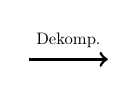
\begin{tikzpicture}
                \draw[->,line width=1pt] (0,0) -- node[midway, above, scale=0.6, yshift=3pt] {Dekomp.} (1,0);
            \end{tikzpicture}
        \end{column}
        
        \begin{column}{0.2\textwidth}

            \begin{minipage}[0.4\textheight]{0.1\textwidth}
                \begin{tikzpicture}[scale=0.3, every node/.style={scale=0.4, circle,fill=TUMGray}, draw=TUMGray]
                    \draw (-4.0,4.3) node[fill=TUMSecondaryBlue] (A) {};
                    \draw (-2.6,3.9) node[fill=TUMSecondaryBlue] (B) {};
                    \draw (-1.8,3.1) node[fill=TUMAccentGreen] (C) {};
                    \draw (-1.2,4.1) node[fill=TUMSecondaryBlue] (D) {};
                    \draw (-5.4,1.9) node[fill=TUMSecondaryBlue] (E) {};
                    \draw (-6.2,2.8) node[fill=TUMAccentOrange] (F) {};
                    \draw (-6.2,1.0) node[fill=TUMAccentOrange] (G) {};
                    \draw (-4.8,0.6) node[fill=TUMAccentOrange] (H) {};
                    \draw (-0.5,0.7) node[fill=TUMAccentGreen] (I) {};
                    \draw (-2.1,-0.4) node[fill=TUMAccentGreen] (J) {};
                    \draw (-0.4,-0.3) node[fill=TUMAccentGreen] (K) {};
                    \draw (-2.2,1.1) node[fill=TUMAccentOrange] (L) {};

                    \node at (-5,3) (AF) {};
                    \node at (-3.5,1.75)  (MID) {};
                    \node at (-2.75,1.75) (NB) {};
                    \node at (-1.5,1.5) (RIGHT) {};
                    \node at (-1,2.5) (CD) {};
                    \draw[line width=1.5+rand] (G) -- node[midway] (GH) {} (H);
                    \draw[line width=1.5+rand] (A) -- (AF) -- (F);
                    \draw[line width=1.5+rand] (GH) -- (MID) -- (AF);
                    \draw[line width=1.5+rand] (E) -- (MID);
                    \draw[line width=1.5+rand] (B) -- (NB);
                    \draw[line width=1.5+rand] (C) -- (CD) -- (D);
                    \draw[line width=1.5+rand] (J) -- node[midway] (JK) {} (K);
                    \draw[line width=1.5+rand] (MID) -- (NB) -- (RIGHT) -- (CD) -- (RIGHT) -- (JK);
                    \draw[line width=1.5+rand] (NB) -- (L);
                    \draw[line width=1.5+rand] (RIGHT) -- (I);
                \end{tikzpicture}
            \end{minipage}

            \vspace{0.5cm}

            \begin{minipage}[0.4\textheight]{0.1\textwidth}
                \begin{tikzpicture}[scale=0.34, every node/.style={scale=0.4, circle,fill=TUMGray}, draw=TUMGray]
                    \draw (-4.0,4.3) node[fill=TUMSecondaryBlue] (A) {};
                    \draw (-2.6,3.9) node[fill=TUMSecondaryBlue] (B) {};
                    \draw (-1.8,3.1) node[fill=TUMSecondaryBlue] (C) {};
                    \draw (-1.2,4.1) node[fill=TUMSecondaryBlue] (D) {};
                    \draw (-5.4,1.9) node[fill=TUMAccentOrange] (E) {};
                    \draw (-6.2,2.8) node[fill=TUMAccentOrange] (F) {};
                    \draw (-6.2,1.0) node[fill=TUMAccentOrange] (G) {};
                    \draw (-4.8,0.6) node[fill=TUMAccentOrange] (H) {};
                    \draw (-0.5,0.7) node[fill=TUMAccentGreen] (I) {};
                    \draw (-2.1,-0.4) node[fill=TUMAccentGreen] (J) {};
                    \draw (-0.4,-0.3) node[fill=TUMAccentGreen] (K) {};
                    \draw (-2.2,1.1) node[fill=TUMAccentGreen] (L) {};


                    \node at (-5,3.5) (AF) {};
                    \node at (-4,2)  (MID) {};
                    \node at (-3,2.25) (NB) {};
                    \node at (-1,2) (RIGHT) {};
                    \node at (-1,3) (CD) {};

                    \draw[line width=1.5+rand] (G) -- node[midway] (GH) {} (H);
                    \draw[line width=1.5+rand] (A) -- (AF) -- (F);
                    \draw[line width=1.5+rand] (GH) -- (MID) -- (AF);
                    \draw[line width=1.5+rand] (E) -- (MID);
                    \draw[line width=1.5+rand] (B) -- (NB);
                    \draw[line width=1.5+rand] (C) -- (CD) -- (D);
                    \draw[line width=1.5+rand] (J) -- node[midway] (JK) {} (K);
                    \draw[line width=1.5+rand] (MID) -- (NB) -- (RIGHT) -- (CD) -- (RIGHT) -- (JK);
                    \draw[line width=1.5+rand] (NB) -- (L);
                    \draw[line width=1.5+rand] (RIGHT) -- (I);

                    \draw[TUMAccentOrange, line width=1pt] (-7,-1.25) rectangle (0,5);
                \end{tikzpicture}	
            \end{minipage}

            \vspace{0.5cm}

            \begin{minipage}[0.4\textheight]{0.1\textwidth}
                \begin{tikzpicture}[scale=0.34, every node/.style={scale=0.4, circle,fill=TUMGray}, draw=TUMGray]
                    \draw (-4.0,4.3) node[fill=TUMAccentOrange] (A) {};
                    \draw (-2.6,3.9) node[fill=TUMSecondaryBlue] (B) {};
                    \draw (-1.8,3.1) node[fill=TUMSecondaryBlue] (C) {};
                    \draw (-1.2,4.1) node[fill=TUMSecondaryBlue] (D) {};
                    \draw (-5.4,1.9) node[fill=TUMSecondaryBlue] (E) {};
                    \draw (-6.2,2.8) node[fill=TUMAccentOrange] (F) {};
                    \draw (-6.2,1.0) node[fill=TUMAccentOrange] (G) {};
                    \draw (-4.8,0.6) node[fill=TUMAccentGreen] (H) {};
                    \draw (-0.5,0.7) node[fill=TUMAccentGreen] (I) {};
                    \draw (-2.1,-0.4) node[fill=TUMAccentOrange] (J) {};
                    \draw (-0.4,-0.3) node[fill=TUMAccentGreen] (K) {};
                    \draw (-2.2,1.1) node[fill=TUMAccentGreen] (L) {};

                    \node at (-5.5,4) (AF) {};
                    \node at (-4,3)  (MID) {};
                    \node at (-3,2.0) (NB) {};
                    \node at (-1.5,2) (RIGHT) {};
                    \node at (-0.5,3) (CD) {};

                    \draw[line width=2.0+rand] (G) -- node[midway] (GH) {} (H);
                    \draw[line width=2.0+rand] (A) -- (AF) -- (F);
                    \draw[line width=2.0+rand] (GH) -- (MID) -- (AF);
                    \draw[line width=2.0+rand] (E) -- (MID);
                    \draw[line width=2.0+rand] (B) -- (NB);
                    \draw[line width=2.0+rand] (C) -- (CD) -- (D);
                    \draw[line width=2.0+rand] (J) -- node[midway] (JK) {} (K);
                    \draw[line width=2.0+rand] (MID) -- (NB) -- (RIGHT) -- (CD) -- (RIGHT) -- (JK);
                    \draw[line width=2.0+rand] (NB) -- (L);
                    \draw[line width=2.0+rand] (RIGHT) -- (I);

                \end{tikzpicture}	
            \end{minipage}

            \vfill
            \hspace{0.5\textwidth} {\LARGE \vdots}
        \end{column}

        \begin{column}{0.1\textwidth}
            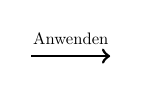
\begin{tikzpicture}
                \draw[->, line width=1pt] (0,0) -- node[above, midway, scale=0.6, yshift=3pt] {Anwenden} (1,0);
            \end{tikzpicture}
        \end{column}
        
        \begin{column}{0.24\textwidth}
            \begin{tikzpicture}[scale=0.4, every node/.style={scale=0.5, circle}]
                \drawgraph
            \end{tikzpicture}	
        \end{column}
    \end{columns}
\end{frame}

\begin{frame}[fragile]{Berechnung der Signaturen}
    \begin{center}
        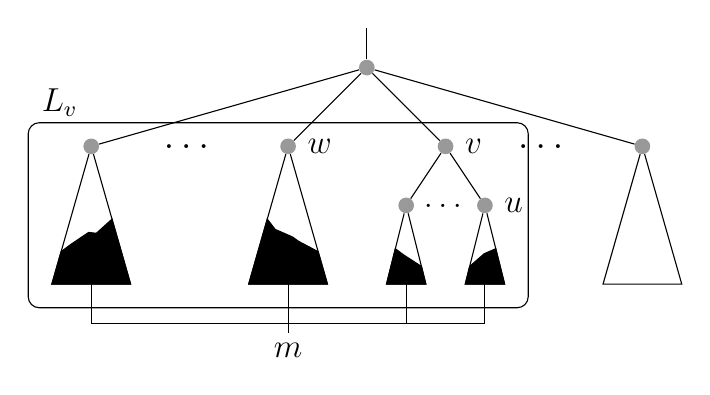
\begin{tikzpicture}[
            mynode/.style={circle, scale=0.6, fill=black!40},
            randomdraw/.style={decoration={random steps, segment length=5pt, amplitude=2.3pt}}
        ]
            \foreach \x/\y/\lbl in {%
                -3.5/0/A,
                -1/0/W,
                1/0/V,
                3.5/0/B,
                0/1/R,
                0.5/-0.75/C,
                1.5/-0.75/U%
            }{
                \node at (\x,\y) [mynode] (\lbl) {};
            }
            
            \foreach \lbl in {A,W,V,B}{
                \path (R) edge (\lbl);
            }
            
            \path (A) -- node[font=\Large]{\ldots} (W);
            \path (V) -- node[font=\Large]{\ldots} (B);
            \path (C) -- node[font=\large]{\ldots} (U);
            
            \draw (C) -- (V) -- (U);
            
            \draw (R) -- (0,1.5);
            
            \foreach \lbl/\lft/\rgt in {U/1.25/1.75,C/0.25/0.75,A/-4/-3,B/3/4,W/-1.5/-0.5}{%
                \path[draw] (\lbl) -- (\lft, -1.75) -- coordinate[midway](\lbl{}M) (\rgt, -1.75) -- (\lbl); 
            }
            
            \foreach \lbl/\n in {W/$w$,V/$v$,U/$u$}{%
                \node [label={0:\large\n}] at (\lbl) {};
            }
            
            \draw[rounded corners] (-4.3,-2.05) rectangle (2.05,0.3);
            \node at (-3.9, 0.55) {\large$L_v$};
            
            \pgfmathsetseed{1}
            \foreach \lbl/\ln/\ls/\rn/\rs/\out/\in in {
                A/-4/near end/-3/midway/30/120,
                W/-1.5/midway/-0.5/near end/20/150,
                C/0.25/midway/0.75/near end/30/120,
                U/1.25/near end/1.75/midway/30/160%
            } {
            
                \path (\lbl) -- coordinate[\ls](\lbl{}L) (\ln, -1.75);
                \path (\lbl) -- coordinate[\rs](\lbl{}R) (\rn, -1.75);
                \draw[fill=black] decorate[randomdraw]{(\lbl{}L) --  (\lbl{}R)} -- (\rn, -1.75) -- (\ln, -1.75) -- cycle; 
            }
            
            
            \draw (-3.5,-2.25) -- node[midway, label={270:\large$m$}](M){} (1.5, -2.25);
            \draw (M.north) -- (M.south);
            \foreach \x in {-3.5,-1,0.5,1.5}{%
                \draw (\x, -1.75) -- (\x, -2.25);
            }
        \end{tikzpicture}
    \end{center}

    \only<2>{
       \begin{equation*}
           \begin{aligned}
               C_v(\vec{g}, m) = \min \{ & C_w(\vec{g}_w, m - x) + C_u(\vec{g}_u, x) \mid \\ & \qquad 0 \leq x \leq m \land \vec{g}_w + \vec{g}_u = \vec{g} \}
           \end{aligned}
       \end{equation*}
    }   

    \only<3>{
        \begin{equation*}
            \begin{aligned}
                C_v(\vec{g}, m) = \weight(e) + \min \{ & C_w(\vec{g}_w, m - n_v) + C_u(\vec{g}_u, n_v - x) \mid \\ & \qquad 1 \leq x \leq \mu \land \vec{g}_w + \vec{g}_u + \vec{e}(x) = \vec{g} \}
            \end{aligned}
        \end{equation*}
    }
\end{frame}
